% !TeX root = ../pythonTutorial.tex
\chapter{Grundlagen}

% !TeX root = ../../pythonTutorial.tex
\section{Was ist Python?}
\label{grundlagen:sec:WasIstPython}
Die Programmiersprache Python wurde Anfang der 1990er Jahre von Guido van Rossum als Universalprogrammiersprache entwickelt.
Der Name der Sprache beruht auf der Komikergruppe Monty Python.
Hierzu lassen sich auch zahlreiche Anspielung in der Dokumentation von Python finden.
Python wurde mit dem Ziel entworfen, eine einfache, gut verst�ndliche und �bersichtliche Programmiersprache zur Verf�gung zu stellen.
Dies soll nicht nur durch eine �bersichtliche Standardbibliothek erreicht werden, sondern auch durch die Modulare Erweiterbarkeit.
Im Folgenden wird die Programmiersprache Python in der Version 3 behandelt.

\section{Installation}

\label{grundlagen:sec:Installation}
Python \randnotiz{Installation} kann auf der Webseite \url{https://www.python.org} f�r eine Vielzahl von Betriebssystemen bezogen werden. 
Es stehen 32- und 64-Bit Versionen zur Verf�gung. 
Nach dem Start des Installationsassistenten wird der Nutzer durch die Installation gef�hrt. 
Der Ablauf der Installation unterscheidet sich je nach Betriebssystemen nur gering bis gar nicht.
Nach erfolgreichem Abschluss stehen dem Anwender verschiedene Programme f�r die Arbeit mit Python zur Verf�gung.
Im vom Nutzer gew�hlten Installationsverzeichnis befinden sich nun folgende Programme: 
\begin{description}
	\item[\textit{IDLE}] Standard IDE\footnote{Integrated Development Environment} f�r Python
	\item[\textit{Python}] Standard Konsolen Interpreter
	\item[\textit{Pythonw}] Standard Interpreter ohne Konsolenausgabe
\end{description}
Diese Programme reichen aus, um Code mit Python zu entwickeln. 
Der Python Interpreter kann in der Konsole mit dem Befehl \lstinline{python} aufgerufen werden. 
Die folgenden Abschnitte beschreiben Besonderheiten bei der Installation auf einzelnen Betriebssystemen. 
\subsection{Hinweis zur Installation unter Windows}
\label{grundlagen:sec:InstallationWindows}
Windows Nutzer m�ssen die Systemvariable f�r Python im Installationsassistenten hinzuf�gen lassen. 
Andernfalls kann Python nur im Installationsverzeichnis bzw. durch die Angabe des kompletten Pfads aufgerufen werden. 
In Abbildung \ref{grundlagen:img:InstallationWindows} ist die notwendige Auswahl zu sehen. 
\begin{figure}[ht]
	\centering
	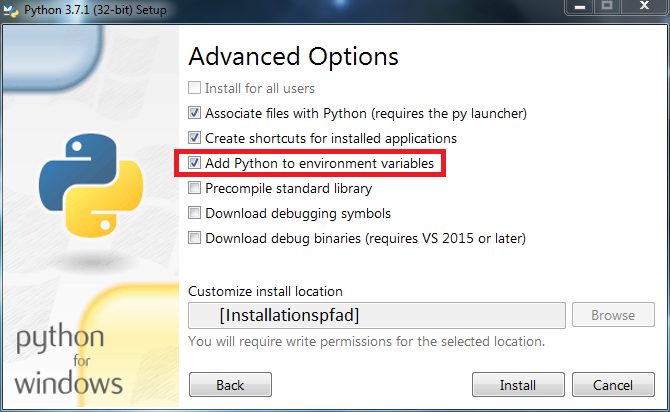
\includegraphics[scale=0.5]{images/InstallationWindows.png}
	\caption{Start des Installationsassistenten}
	\label{grundlagen:img:InstallationWindows}
\end{figure}
%
\subsection{Hinweis zur Installation unter Mac}
\label{grundlagen:sec:InstallationMac}
Im Folgenden wird die Installation unter macOS X gezeigt.

\begin{figure}[ht]
	\centering
	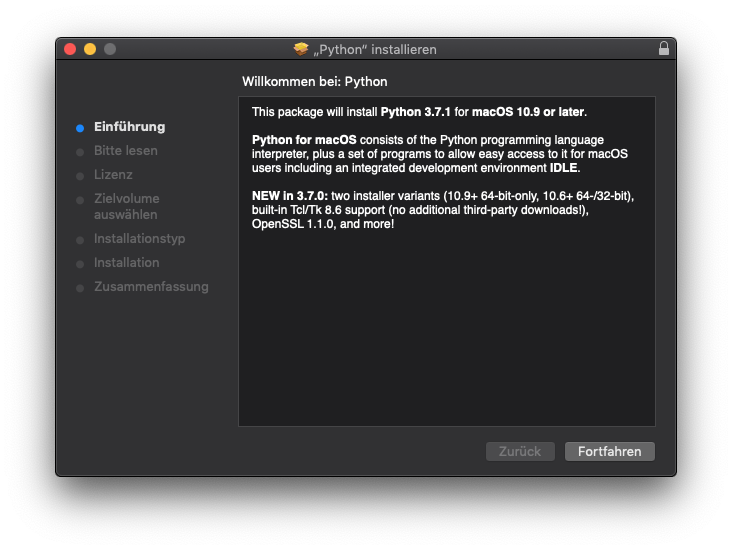
\includegraphics[scale=0.5]{images/InstallationMac.png} 
	\caption{Start des Installationsassistenten}
	\label{grundlagen:img:InstallationMac}
\end{figure}
Nach Ende der Installation befindet sich der Python Ordner im Finder (Dateiexplorer).

\begin{figure}[ht]
	\centering
	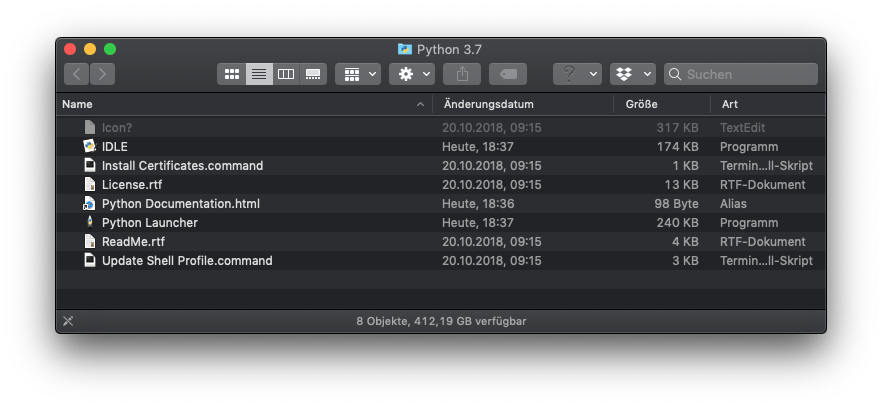
\includegraphics[scale=0.5]{images/PythonFinder.png} 
	\caption{Fertige Installation}
	\label{grundlagen:img:FinishInstall}
\end{figure}
Zuletzt wurde durch den Assistent unter \texttt{/Library/Frameworks/\\Python.framework} noch das Python Framework abgelegt.
Ohne das w�re die Arbeit mit Python unter Mac nicht m�glich.

\subsection{Hinweis zur Installation unter Linux(Ubuntu)}
\label{grundlagen:sec:InstallationLinux}
In diesem Kapitel wird die Installation f�r Ubuntu Version 18.04.1 LTS erl�utert.
Im Gegensatz zu den anderen Betriebssystemen, wird hier nur der Python Interpreter in der Version 3.6.6 mitgeliefert
Standard Entwicklungsumgebung IDLE ist nicht vorinstalliert.
Diese kann �ber das Paket IDLE nachtr�glich installiert werden.
Sollte die Arbeit mit Python noch nicht m�glich sein, kann durch den folgenden Befehl die Installation manuell angesto�en werden.

\begin{lstlisting}[language=BASH, label={grundlagen:lst:InstallationLinux}]
sudo apt-get install python3 python-doc
\end{lstlisting}

Diese Installation umfasst unter anderem auch die Dokumentation von Python.
Nach Abschluss der Installationsroutine kann wie mit jedem anderen Betriebssystem mit Python gearbeitet werden.

\section{Python Interpreter} 
\label{grundlagen:sec:Interpreter}
Die einfachste M�glichkeit, Python Code auszuf�hren, ist die direkte �bergabe des Codes an den sogenannten Python Interpreter. 
Dabei handelt es sich um eine Konsolenanwendung, die Code ausf�hren und gegebenenfalls auftretende Ergebnisse ausgeben kann. 
Dabei kann ein Nutzer den Code entweder direkt in die Konsole eingeben oder aus einer Datei auslesen lassen. 
Wie bei anderen Programmiersprachen auch, stehen f�r Python verschiedene IDEs zur Verf�gung, welche in Kapitel \ref{ides:section:ides} behandelt werden. 
F�r die ersten Versuche mit Python reicht der Interpreter jedoch v�llig aus. Dieser wird standardm��ig mit Python installiert.

In Abbildung \ref{grundlagen:img:Interpreter} ist der Interpreter zu sehen. 
Zus�tzlich zur Version werden auch noch der Herausgeber von Python sowie die Uhrzeit angezeigt.
Bereits jetzt kann erster Code ausgef�hrt werden.
Im Folgenden werden zu einzelnen Bestandteilen von Python Beispiele beigef�gt, die leicht im Interpreter ausf�hrbar sind. 
Es wird dem Leser empfohlen, sie zum besseren Verst�ndnis nachzuvollziehen, falls m�glich durch selbst�ndiges Ausprobieren.

\begin{figure}[ht]
	\centering
	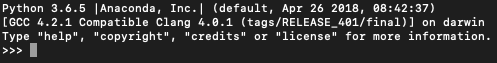
\includegraphics[width=0.8\textwidth]{images/Interpreter.png} 
	\caption{Ansicht nach Start des Interpreters}
	\label{grundlagen:img:Interpreter}
\end{figure}

\subsection*{Interaktiver Modus} 
\label{grundlagen:sec:InteraktiverModus}
Wird der Interpreter ohne Angabe einer Quellcodedatei gestartet, befindet dieser sich im interaktiven Modus. 
Der Nutzer kann hier direkt Anweisungen eingeben. Durch die Ausgabe der Zeichen $>>>$ zeigt die Konsole an, dass sie eine Anweisung erwartet. 
In Python existieren auch mehrzeilige Anweisungen. 
Nach der Eingabe der ersten Zeile werden die Zeichen $...$ ausgegeben, was bedeutet, dass Folgeanweisungen erwartet werden. 
\subsection*{Einlesen einer Datei}
\label{grundlagen:sec:EinlesenDatei}
Auf Dauer ist die direkte �bergabe des Codes an den Interpreter sehr unpraktisch. 
Um Code erneut nutzen zu k�nnen und zu speichern, kann dieser in Dateien abgelegt werden.
Dies kann mit einem simplen Texteditor erfolgen.
Dateien, die Python Code enthalten, werden mit der Dateiendung ''.py'' gekennzeichnet. 
Sie k�nnen direkt mit dem der Konsole ausgef�hrt werden.
Dazu muss Python der relative Pfad der Pythondatei (.py-Endung) �bergeben werden.  
\begin{lstlisting}[language=BASH, label={grundlagen:lst:BashStartPython1}]
python <Relativer Dateipfad der Pythondatei>
\end{lstlisting} 
Da nur der relative Pfad angegeben werden muss, muss lediglich der Dateiname angegeben werden, falls die Konsole sich bereits im selben Verzeichnis wie die zu �ffnende Datei befindet.
\section{Syntax}
\label{grundlagen:sec:Syntax}
Im \randnotiz{Syntax} Folgenden werden wichtige Grundkonzepte der Programmiersprache\\ \mbox{Python} erl�utert.
%Benoetigt um korrekten Zeilenumbruch zu erzwingen
\subsection{Allgemeine Strukturen}
\label{grundlagen:sec:AllgemeineStrukturen}
Anders als bei anderen Programmiersprachen wie beispielsweise Java oder C++, ben�tigt Python keine Klassenkonstrukte oder main-Methoden zur Ausf�hrung. 
Das bedeutet, dass einzelne Anweisungen in Python korrekt ausgef�hrt werden k�nnen. 
Sollten f�r die Bearbeitung von komplexeren Problemen objektorientierte Ans�tze ben�tigt werden, kann auch dies mit Python umgesetzt werden. 
Weitere Informationen zur Objektorientierung mit Python finden sich im weiteren Verlauf des Python Tutorials.
F�r den Moment reicht es f�r den Leser zu wissen, dass Anweisungen bereits zeilenweise ausgef�hrt werden k�nnen. 
Das kann sehr simpel getestet werden, indem der Python Interpreter als einfacher Taschenrechner genutzt wird. 
In Abbildung \ref{grundlagen:img:AusdrueckeInInterpreter} wird dies gezeigt. Einfache Ausdr�cke wie Summen, Subtraktionen, Multiplikationen und Divisionen k�nnen direkt eingegeben werden. 
Nach Bet�tigung der Eingabe-Taste liefert Python das Ergebnis des Ausdrucks.\\
\begin{figure}
	\centering
	\includegraphics[width=1\textwidth]{images/AusdrueckeInInterpreter.png} 
	\caption{Einfache Ausdr�cke im Python Interpreter}
	\label{grundlagen:img:AusdrueckeInInterpreter}
\end{figure}
\subsection{Leerzeichen und Einr�ckung}
\label{grundlagen:sec:LeerzeichenEinrueckung}
Um in Python Bl�cke auszuzeichnen, werden im Gegensatz zu Java oder C++ keine geschweiften Klammern genutzt.
In Python werden Bl�cke durch das Einr�cken der Zeilen markiert. 
Hierf�r sind entweder der Tabulator oder vier aufeinander folgende Leerzeichen vorgesehen.
\subsection{Kommentare}
\label{grundlagen:sec:Kommentare}
Innerhalb der Programmiersprache Python wird zwischen Zeilen- und Blockkommentaren unterschieden.
Zeilenweise Kommentare werden durch das Rautensymbol \lstinline$\#$ eingeleitet.
Blockkommentare hingegen werden durch drei aufeinander folgende Anf�hrungszeichen \lstinline$"""$ jeweils zu Beginn und am Ende des Kommentars markiert.
Hier wird jeweils ein Beispiel gezeigt:

\lstinputlisting[language=Python,label={grundlagen:lst:Kommentare}]{chapters/basics/src/comment.py}
\subsection{Typsicherheit}
\label{grundlagen:sec:Typsicherheit}
Anders als bei Java und C++ ist Python eine nur schwach typisierte Sprache.
Somit ist bei der Initialisierung keine Typangabe erforderlich.
Der Datentyp wird beim Initialisieren dynamisch ermittelt und automatisch zugewiesen.
Um einer Variable trotzdem einen gew�nschten Typ zuzuweisen, kann man sie einfach mit dem entsprechenden Typ initialisieren.
Weitere Informationen zu Datentypen werden in Abschnitt \ref{basicdatatypes:sec:ElementareDatentypen} erl�utert.
\section{Beispiel \glqq Hello World!\grqq}
\label{grundlagen:sec:HalloWorld}
Einfache \randnotiz{Beispiel} Ausgaben k�nnen mit der print()- Anweisung gemacht werden. 
Innerhalb der Klammern muss ein String �bergeben werden, sprich eine einfache Zeichenkette. 
Diese wird durch umschlie�ende einfache oder doppelte Anf�hrungszeichen markiert (''EinString''/'EinString'). 
Der Einfachheit halber, wird hier noch auf die genaue Erkl�rung der einzelnen Bestandteile der Anweisung verzichtet. 
Ein einfaches ''Hello-World!''-Programm ben�tigt in Python nur eine Zeile: 
\lstinputlisting[language=python, label={grundlagen:lst:HalloWorld}]{chapters/basics/src/helloworld.py} 
Es handelt sich dabei um ein vollst�ndiges Python-Programm, das in dieser Form ausgef�hrt werden kann. 
Wie bereits erl�utert, werden anders als bei Java oder C++ keine Klassenkonstrukte oder main-Methoden ben�tigt.

%\uebung
%\aufgabe{grundlagen01} 
%\aufgabe{grundlagen02}

\uebungTutorial{grundlagen01}{grundlagen02}


% !TeX root = ../../pythonTutorial.tex


\section{IDEs}

Python Programmierung mit der IDLE (in Python integrierte Entwicklungsumgebung) oder Python Shell sind gute M�glichkeiten um den Einstieg in Python  zu vereinfachen. Ein grunds�tzliches Verst�ndnis der Sprache und erste kleine Programme lassen sich so bew�ltigen. Sobald jedoch gr��ere Programme oder Projekte anstehen kann es mit diesen Tools schnell frustrierend werden.

Eine passende IDE (Integrierte Entwicklungsumgebung) oder selbst ein einfacher Code-Editor kann einem das leben deutlich vereinfachen. Im folgenden werden einige geeigneten IDEs f�r Python vorgestellt und f�r jede einige Vor- und Nachteile aufgezeigt.

\textbf{Was ist eine IDE?}

Integrierte Entwicklungsumgebungen vereinen wichtige Tools f�r das Erstellen von Software unter einer Oberfl�che. Dazu z�hlen Editor mit Syntaxhervorhebung, Compiler, Debugger, Interpreter und weitere Werkzeuge, die dem Entwickler die Arbeit erleichtern.

Durch den Austausch zwischen Werkzeugen innerhalb der IDE k�nnen Arbeitsg�nge erleichtert und beschleunigt werden. Fehler im Quelltext beispielsweise k�nnen direkt in der entsprechenden Zeile markiert werden.

\textbf{Anforderungen an eine geeignete Python Entwicklungsumgebung}

Es gibt ein paar Grundanforderungen an eine geeignete oder gute Python Entwicklungsumgebung:

\begin{description}
\item[Debugging Unterst�tzung]\hfill \\
Schrittweise durch den Code zu wandern, w�hrend dieser ausgef�hrt wird, ist eine weiter Grundaufgabe einer IDE.
\item[Syntax Highlighting]\hfill \\
Farbliche Markierungen erleichtern die Suche nach bestimmten Keywords. Die Lesbarkeit des Codes wird hierdurch verbessert.
\item[Automatische Codeformatierung]\hfill \\
Eine gute IDE erkennt das Zeilenende beispielsweise nach einem \textit{While-Statement} und r�ckt die n�chste Zeile automatisch ein.
\item[Ausf�hren des Codes innerhalb der IDE]\hfill \\
Wenn der Code au�erhalb der IDE ausgef�hrt werden muss, ist es eher ein Text-Editor als eine IDE.
\item[Interaktive Console]\hfill \\
Live Ein- und Ausgabe einzelner Codezeilen.
\item[Fehlererkennung]\hfill \\
Syntaxfehler sollten automatisch markiert werden und Runtime-Fehler genannt werden.
\end{description}

\subsection{Einige IDEs vorgestellt}
\textbf{Eclipse} \\
Wer schon mit Java programmiert hat, ist wohl schon mal auf Eclipse gesto�en. Durch die Installation von PyDeth l�sst sich Eclipse gut (und kostenlos) f�r die Python-Entwicklung erweitern und bietet dabei wichtige Features, wie zum Beispiel Code Completion, Python Debugging, eine interaktive Python Konsole oder das Einbinden von Django.

\textbf{Vorteile:}
Wenn Eclipse bereits auf dem Rechner vorhanden ist, gen�gt der Download der PyDeth Erweiterung, welche nach einem Neustart von Eclipse sofort eingebunden ist.

\textbf{Nachteile:}
Der Einstieg in die Python Programmierung f�r Eclipse-Neulinge kann in der sehr gro�en Entwicklungsumgebung Eclipse zu Schwierigkeiten f�hren.

\textbf{Visual Studio} \\
Die IDE aus dem Hause Microsoft bietet viele eigene Erweiterungen und Entwicklungs-Features an, welche dem Entwickler eine gute Individualisierungsm�glichkeit bieten. Die Visual Studio Python Tools erm�glichen es, alle �blichen Entwicklungsm�glichkeiten bei Programmierung mit Python zu nutzen. Visual Studio ist sowohl in der Community-Version umsonst, aber auch in einem Bezahlmodell verf�gbar.

Visual Studio Community kann kostenlos �ber folgenden Link heruntergeladen werden: https://visualstudio.microsoft.com/de/vs/community/

\textbf{Nachteile:}
Der Download ausschlie�lich f�r die Python-Programmierung ist recht gro� (3-4GB). Es m�ssen sowohl das Programm an sich, als auch die Python-Erweiterung heruntergeladen werden. Visual Studio ist ausschlie�lich f�r Windows und MacOs verf�gbar. Eine Linux-Variante wird allerdings von Visual Studio Code angeboten. Vergleichbar mit Eclipse ist auch Visual Studio nicht sonderlich einsteigerfreundlich.

\textbf{Atom}  \\
Etwas schlichter geht es im Atom Editor zu. Das klare und strukturierte Interface ist auch f�r Einsteiger gut verst�ndlich und dient daher als geringere H�rde, die ein Neuling �berwinden muss, als die �berladenen Interfaces von Eclipse oder Visual Studio. Python kann durch eine Erweiterung nachtr�glich installiert werden, welche w�hrend der Laufzeit hinzugef�gt werden kann.

\textbf{Vorteile:}
Einsteigerfreundliche Alternative mit geringem Download- und Installationsumfang, sowie Plattformunabh�ngigkeit.

\textbf{Nachteile:}
\textit{Build-} und \textit{Debugging-Support} sind keine eingebauten Features, sondern nur als Community-Addon verf�gbar.


\textbf{PyCharm} \\
PyCharm ist (wie es der Name vermuten l�sst) eine IDE explizit f�r Python. Es ist neben der Hauptdatei keine Erweiterung n�tig, ein neues Projekt kann sofort gestartet und mit dem Programmieren sofort begonnen werden. PyCharm ist Plattformunabh�ngig und sowohl in einer freien Open-Source-Version nutzbar, als auch in einer kostenpflichtigen Pro-Version erh�ltlich.

\textbf{Vorteile:}
PyCharm bietet einen vielf�ltigen Support an und eine sehr aktive Community. Egal an welcher Stelle man ein Problem hat, es wird einem mit gro�er Wahrscheinlichkeit geholfen.  

\textbf{Nachteile:}
Die Ladezeiten sind vergleichbar lang und an manchen Stellen finden sich kleinere Usability-Schwachpunkte.


% !TeX root = ../../pythonTutorial.tex

\section{Elementare Datentypen}
\label{basicdatatypes:sec:ElementareDatentypen}

�hnlich wie bei Java und C oder C++ gibt es auch in Python Variablen. Allerdings gibt es dabei immense Unterschiede zu den anderen Programmiersprachen, weshalb sich ein genauerer Blick auf die einzelnen Datentypen in jedem Fall lohnt. Bei vielen bekannten Sprachen wird einer Variablen ein bestimmter Datentyp zugeordnet (deklariert). Der Datentyp kann darauf folgend zur Laufzeit nicht wieder ge�ndert werden, der Wert innerhalb des Datentyps allerdings schon. So lassen sich in eine Variable des Typ Integer beispielsweise keine String-Werte speichern. In Python hingegen ist dies ohne weiteres m�glich. Hier wird g�nzlich auf eine explizite Typdeklaration verzichtet. Zeigt eine Variable beispielsweise auf eine ganze Zahl, so wird diese als ein Objekt vom Typ Integer interpretiert. Allerdings ist es m�glich, diese im n�chsten Schritt einfach auf ein String-Objekt zeigen zu lassen. Dies ist in Python m�glich, weil eine Variable ein Objekt lediglich referenziert und dadurch keinem Typ zugewiesen wird.\\
Betrachten wir nun die Datentypen etwas genauer.

\subsection{Zahlenoperatoren}
\label{basicdatatypes:sec:Zahlenoperatoren}

Da in Python auf Typdeklaration verzichtet wird, muss dies beim Anlegen von Variablen nicht ber�cksichtigt werden. Wird eine ganze Zahl (Integer) ben�tigt, kann diese, falls n�tig, auch in eine Gleitkommazahl (float) umgewandelt werden, ohne viel am Code zu �ndern. Python deklariert im Hintergrund selbst und spart so unn�tige Komplexit�ten und Fehlerquellen. (Beispiel \ref{refzahl})

\begin{lstlisting}[label=refzahl]
# Zahlenoperatoren
i = 42
type(i)
// Ausgabe: <class 'int'>
i = 42.22
type(i)
// Ausgabe: <class 'float'>
\end{lstlisting}

\textbf{Boolean}

Boolean gibt an, ob ein Statement \textit{true} oder \textit{false} ist. Dadurch lassen sich Fallunterscheidungen oder Abfragen erm�glichen. (Beispiel in Listing \ref{basicDatatypes:lst:refbool})

\begin{lstlisting}[label=basicDatatypes:lst:refbool]
# Boolean
i = True
i
// Ausgabe: True

\end{lstlisting}

\textbf{String}

Der String ist eine Zeichenkette, also eine Aneinanderreihung von verschiedenen Zeichen. Dazu z�hlen W�rter, aber auch beispielsweise Hexadezimal-Codes oder E-Mail Adressen.

Wie in den meisten objektorientierten Programmiersprachen lassen sich auch in Python die einzelnen Zeichen eines Strings abrufen, indem der dazugeh�rige Index abgefragt wird.

Wie in Listing \ref{basicDatatypes:lst:refstring} kann die L�nge des gesamten Strings durch einfache Abfrage angezeigt werden.

\begin{lstlisting}[label=basicDatatypes:lst:refstring]
# Strings
i = "Python"
print (i)
// Ausgabe: Python

print(i[0])
// Ausgabe: P

print(len(i))
// Ausgabe: 6

\end{lstlisting}

\subsection{ENUMs}
\label{basicdatatypes:sec:Enums}

Enums dienen in den objektorientierten Programmiersprachen zur Aufz�hlung von Ausdr�cken einer endlichen Menge. So werden zum Beispiel Jahreszeiten, Monate oder Farben oft als Enums umgesetzt (vgl. Listing \ref{refenum}).


\begin{lstlisting}[label=refenum]
# Enums
from enum import Enum
class Color(Enum):
    RED = 1
    GREEN = 2
    BLUE = 3

\end{lstlisting}

\subsection{NULL oder NONE}
\label{basicdatatypes:sec:NullNone}
Das Schl�sselwort \textit{NULL} wird in vielen Programmiersprachen genutzt. Die Idee dahinter ist einer Variable ein neutrales Verhalten zu geben. Das �quivalent zu \textit{NULL} in Python ist \textit{NONE}. Der Vorteil ist, dass \textit{NONE} exakt der Aufgabe des Schl�sselworts entspricht. Ein Anwendungsfall f�r \textit{NONE} w�re beispielsweise um zu �berpr�fen, ob die Verbindung zu einer Datenbank aufgebaut werden konnte oder nicht (Siehe Beispiel \ref{refnone}).

\begin{lstlisting}[label=refnone]
# NULL oder NONE
database_connection = None

try:
    database = MyDatabase(host, user, password, database)
    database_connection = database.connect()
except DatabaseException:
    pass

if database_connection is None:
// Solange die Variable "NONE", keine Verbindung aufgebaut
    print('The database could not connect')
else:
    print('The database could connect')

\end{lstlisting}

\subsection{Referenz, Identit�t und Kopie}
\label{basicdatatypes:sec:Referenzen}

Wie bereits erw�hnt wurde, wird in Python eine Variable keinem Typ zugewiesen. Zeigt eine Variable jedoch st�ndig auf ein neues Objekt, sind Verwechslungen innerhalb des Codes m�glich. Um dies zu vermeiden bietet sich die Identit�tsfunktion id() an. Diese hilft uns dabei, die verschiedenen Instanzen voneinander zu unterscheiden. Jede Instanz hat dabei unabh�ngig von ihrem Wert und ihrem Typ eine eindeutige Identit�t. \\

Dies ist in Python m�glich, weil eine Variable ein Objekt lediglich referenziert und dadurch keinem Typ zugewiesen wird.

\uebung
\aufgabe{DatatypesAufgabe1}

%\uebungTutorial{DatatypesAufgabe1} 


% !TeX root = ../../pythonTutorial.tex

\section{Kontrollstrukturen}

Die Kontrollstrukturen in Python haben einen formalen Unterschied zu Java oder C++, funktional allerdings sind sie identisch. In Python werden keine geschweiften Klammern genutzt, um die Bl�cke der einzelnen Abfragen abzugrenzen. Dazu gen�gt das Einr�cken der Anweisung. Dies gilt sowohl f�r Bedingungen und Conditional Expressions, als auch f�r Schleifen. Im Folgenden schauen wir uns die einzelnen Strukturen im Detail und mit Beispielen an.

\subsection{If-then-else}

Die if-then-else-Struktur erm�glicht es, wie wir es bereits kennen, simple wenn-dann Abfragen zu t�tigen.\\
Mehrere Abfragem�glichkeiten werden mit elif markiert. Vergleich hierzu Listing \ref{kontrollstrukturen:lst:refif}.



\begin{lstlisting}[label=kontrollstrukturen:lst:refif]
# If-then-else
if statement1:
	print("Fall 1")
elif statement2:
	print("Fall 2")
else:
	print("Fall 3")
\end{lstlisting}

\textbf{Conditional Expressions}

Die Conditional Expressions (engl. bedingte Ausdr�cke) stellen eine kompaktere Schreibweise als if-then-else-Bedinungen dar. Ein Beispiel ist in Listing \ref{kontrollstrukturen:lst:refcond} zu finden. 

\begin{lstlisting}[label=kontrollstrukturen:lst:refcond]
# Conditional Expressions
# Klassisches If-Else
if wort == "start":
	x = "los"
else:
	x = halt"
	
# If-Else als Conditional Expression
x = ("los" if wort == "start" else "halt")

\end{lstlisting}


\subsection{Schleifen}

Python hat sowohl bedingte, als auch Z�hler-Schleifen, welche wir uns beide im Folgenden genauer ansehen werden (vgl. Listing \ref{kontrollstrukture:lst:refwhile} und \ref{kontrollstrukture:lst:reffor}). Schleifen bestehen aus einer Anweisung und einem Kontrollblock, welcher solange durchlaufen wird, bis die Anweisung oder ein Abbruchkriterium erf�llt wurde. Schleifen, die niemals ein Abbruchkriterium erf�llen und so endlos durchlaufen werden, hei�en Endlosschleifen. Diese f�hren dazu, dass der Interpreter irgendwann aufgibt und abbricht.

\begin{lstlisting}[label=kontrollstrukture:lst:refwhile]
# While-Schleife
while Bedingung:
	Anweisungsblock
	if Bedingung:
		Anweisungsblock
		continue
	if Bedingung:
		Anweisungsblock
		break
	Anweisungsblock

\end{lstlisting}

\begin{lstlisting}[label=kontrollstrukture:lst:reffor]
# While-Schleife
for Variable in Objekt:
	Anweisungsblock
	if Bedingung:
		Anweisungsblock
		continue
	Anweisungsblock
	if Bedingung:
		Anweisungsblock
		break
	Anweisungsblock

\end{lstlisting}



\subsection{Ausdr�cke und Operatoren}

Die meisten Operatoren f�r Zahlenwerte sind in Python �hnlich wie bei anderen Programmiersprachen. Im folgenden wird eine �bersicht gegeben.

\begin{table}[h]

\begin{tabular}{|p{0.15\textwidth}|p{0.5\textwidth}|p{0.25\textwidth}|}
\hline
\multicolumn{1}{|c|}{\textbf{Operator}} & \multicolumn{1}{c|}{\textbf{Bezeichnung}} & \multicolumn{1}{c|}{\textbf{Beispiel}} \\ \hline
\hline
+, - & Addition, Subtraktion & 4 - 3 \\ \hline
*, \% & Multiplikation, Rest & 24 \% 5 \newline Ergebnis: 4 \\ \hline
/ & Division & 10 / 3 \newline Ergebnis: 3.33333333333335 \\ \hline
// & Ganzzahldivision & 10 // 3 \newline Ergebnis: 3 \\ \hline
+x, -x & Vorzeichen & -5 \\ \hline
** & Exponentiation & 2 ** 4 \newline Ergebnis: 16 \\ \hline 
or, and, not & Boolsches Oder / Und / Nicht & (a or b) and c \\ \hline
in & Element von & 1 in [1,2,3]  \\ \hline
<, <=, >, >=, !=, == & Vergleichsoperatoren & 4 <= 5 \\ \hline
\end{tabular}
\caption{Ausdr�cke und  Operatoren}

\end{table}




% !TeX root = ../../pythonTutorial.tex
\section{Collections}
\label{collections:sec:collections}

In Python 3 existieren nativ die vier Datenstrukturen List, Tuple, Set und Dictionary, welche im Folgenden vorgestellt werden.

\subsection{List}
\label{collections:sec:list}
\randnotiz{List}

Die Datenstruktur List bietet einen geordneten und ver�nderbaren Beh�lter f�r Python-Objekte, der Duplikate von Elementen erlaubt. Da eine List immer sortiert ist, k�nnen einzelne Elemente aus der Datenstruktur �ber den entsprechenden Index ausgew�hlt und ver�ndert werden. Python unterst�tzt intern keine Arrays, alternativ hierzu kann eine List verwendet werden.

Eine List kann wie folgt initialisiert werden:
\lstinputlisting[language=Python]{chapters/basics/src/list/ListInit.py}
\label{collections:lst:listinit}

Dabei kann sie jegliche Art von Objekten beinhalten; der Datentyp spielt hierbei keine Rolle. 

Beispiel:
\lstinputlisting{chapters/basics/src/list/ListDataType.py}
\label{collections:lst:listdatatype}

Im Gegensatz zu Java und C++ muss der Programmierer darauf achten und sicherstellen, dass die Datenstruktur mit Werten des entsprechenden Datentyps bef�llt wird, um Fehler aufgrund unterschiedlicher Datentypen zu vermeiden.

Der Inhalt einer List kann �ber die \lstinline$print()$-Methode ausgegeben werden. Im folgenden Beispiel werden verschiedene Elemente der List auf der Konsole ausgegeben.
Wird die List als Parameter gew�hlt, wird der Inhalt ausgegeben.
\lstinputlisting{chapters/basics/src/list/ListPrint.py}
\label{collections:lst:listprint}

Wie zuvor erw�hnt, �hnelt die Verwaltung einer List der eines Arrays aus Java oder C++. Durch die Verwendung eines Index k�nnen einzelne Elemente ausgew�hlt oder ver�ndert werden.
\lstinputlisting{chapters/basics/src/list/ListIndex.py}
\label{collections:lst:listindex}

Python erlaubt die Nutzung von negativen Indizes. Mit diesen kann der Inhalt der List in umgekehrter Reihenfolge ausgegeben werden. Ein Index von \lstinline$-1$ wird dem letzten Element der List zugeordnet, \lstinline$-2$ dem vorletzten.
\lstinputlisting{chapters/basics/src/list/ListNegativeIndex.py}
\label{collections:lst:lsitnegativeindex}

In Python existiert f�r die Datenstruktur List keine Methode, die mit \\ \lstinline$contains()$ in Java oder der \lstinline$find()$ aus C++ vergleichbar ist. Stattdessen stehen die Membership Operatoren \lstinline$in$ oder \lstinline$not$ \lstinline$in$ zur Verf�gung, die auf eine beliebige Sequenz oder die hier beschriebenen Collections angewendet, Auskunft dar�ber gibt, ob das spezifizierte Element darin enthalten ist.
\lstinputlisting{chapters/basics/src/list/ListInOperator.py}
\label{collections:lst:listinoperator}
    
Der Python Interpreter stellt nativ einige Funktionen zur Verf�gung. Eine davon ist die \lstinline$len()$-Methode, die die Anzahl an Elementen in einem Objekt liefert.
\lstinputlisting{chapters/basics/src/list/ListLen.py}
\label{collections:lst:listlen}
    
Das \lstinline$del$-Statement erlaubt das L�schen einzelner Elemente oder der gesamten List.
\lstinputlisting{chapters/basics/src/list/ListDelete.py}
\label{collections:lst:listdel}
    

\subsubsection{Methoden einer List}
\label{collections:sec:listmethodes}
\randnotiz{List-Methoden}

\textbf{append():}
F�gt am Ende der List ein Objekt hinzu.
\lstinputlisting{chapters/basics/src/list/ListAppend.py}
\label{collections:lst:listappend}

\textbf{clear():}
Entfernt s�mtliche Objekte aus der List.
\lstinputlisting{chapters/basics/src/list/ListClear.py}
\label{collections:lst:listclear}

\textbf{copy():}
Liefert eine Kopie der List.
\lstinputlisting{chapters/basics/src/list/ListCopy.py}
\label{collections:lst:listcopy}
    
%\newpage
\textbf{count():}
Liefert die Anzahl des spezifizierten Objekts in der List.
\lstinputlisting{chapters/basics/src/list/ListCount.py}
\label{collections:lst:listcount}

\textbf{extend():} 
F�gt der \lstinline$liste1$ den Inhalt der \lstinline$liste2$ am Ende hinzu.
\lstinputlisting{chapters/basics/src/list/ListExtend.py}
\label{collections:lst:listextend}
    
\textbf{index():}
Liefert den Index der Position, an der sich das erste spezifizierte Objekt in der List befindet.
\lstinputlisting{chapters/basics/src/list/ListIndexMethode.py}
\label{collections:lst:listindexmethode}
    
\textbf{insert():}
F�gt ein Objekt an der gew�hlten Position der List hinzu.
\lstinputlisting{chapters/basics/src/list/ListInsert.py}
\label{collections:lst:listinsert}

\textbf{pop():}
Entfernt das Objekt, das sich an der durch den Index spezifizierten Position befindet.
\lstinputlisting{chapters/basics/src/list/ListPop.py}
\label{collections:lst:listpop}
    
\textbf{remove():}
Entfernt das erste Objekt der List, das der Spezifikation entspricht.
\lstinputlisting{chapters/basics/src/list/ListRemove.py}
\label{collections:lst:listremove}
    
\textbf{reverse():}
Invertiert die Folge der Objekte in der List.
\lstinputlisting{chapters/basics/src/list/ListReverse.py}
\label{collections:lst:listreverse}

\textbf{sort():}
Sortiert die List.
\lstinputlisting{chapters/basics/src/list/ListSort.py}
\label{collections:lst:listsort}

    
\subsection{Tuple}
\label{collections:sec:tuple}
\randnotiz{Tuple} 

Ein Tuple stellt einen geordneten und unver�nderbaren Beh�lter f�r Python-Objekte dar. Dieser erlaubt, wie eine List, Duplikate und den Zugriff auf einzelne Elemente �ber einen Index. Tuple sind Datenstrukturen, die ausschlie�lich gelesen werden k�nnen.

Ein Tuple wird mit folgender Syntax erzeugt:
\lstinputlisting{chapters/basics/src/tuple/TupleInit.py}
\label{collections:lst:tupleinit}

Es ist m�glich, leere Tuple zu erzeugen. Wie zuvor erw�hnt, ist deren Inhalt unver�nderlich.

\subsubsection{Arbeiten mit einem Tuple}
\label{collections:sec:workwithtuple} 

Der Inhalt eines Tuple kann, analog zur List, auf der Konsole ausgegeben werden. Das Zuweisen eines neuen Objekts mittels Index f�hrt im Gegensatz zur List zu einem Fehler.
\lstinputlisting{chapters/basics/src/tuple/TupleIndex.py}
\label{collections:lst:tupleindex}    
    
Die Verwendung der Operatoren \lstinline$in$ und \lstinline$not in$ ist, wie die \lstinline$len()$-Methode, analog zur List-Datenstruktur.
\lstinputlisting{chapters/basics/src/tuple/TupleInLen.py}
\label{collections:lst:tupleinlen} 
    
Das \lstinline$del$-Statement erlaubt das L�schen des Tuple. Aufgrund der Unver�nderbarkeit der Datenstruktur k�nnen keine einzelnen Elemente entfernt werden.
\lstinputlisting{chapters/basics/src/tuple/TupleDelete.py}
\label{collections:lst:tupledelete}      

\subsubsection{Methoden eines Tuple}
\label{collections:sec:tuplemethodes}
\randnotiz{Tuple-Methoden}

\textbf{count():}
Liefert die Anzahl des gew�hlten Werts in einem Tuple.
\lstinputlisting{chapters/basics/src/tuple/TupleCount.py}    
\label{collections:lst:tuplecount}  

\textbf{index():}
Liefert die Position des ersten Werts, der mit dem spezifizierten Wert �bereinstimmt.
\lstinputlisting{chapters/basics/src/tuple/TupleIndexMethode.py}
\label{collections:lst:tupleindexmethode}  

\subsection{Set}
\label{collections:sec:set}
\randnotiz{Set} 

Ein Set ist durch das Hinzuf�gen oder Entfernen von Objekten ver�nderbar und erlaubt keine Duplikate. Das Initialisieren mit mehrfach identischen Werten f�hrt nicht zu einem Fehler, jedoch werden die �berz�hligen Werte aus dem Set entfernt. Die enthaltenen Elemente sind unver�nderlich. Zudem ist die Datenstruktur ungeordnet, weshalb nicht auf einzelne Objekte mittels Index zugegriffen werden kann. 

Ein Datenbeh�lter vom Typ Set kann mit folgender Syntax erzeugt werden:
\lstinputlisting{chapters/basics/src/set/SetInit.py}
\label{collections:lst:setinit}  
    
\subsubsection{Arbeiten mit Sets}
\label{collections:sec:workwithset}
Bei der Ausgabe eines Set auf der Konsole ist die Reihenfolge der Elemente nicht garantiert. 

% Wird der Inhalt eines Sets auf der Konsole ausgegeben, erscheint die Reihenfolge der Elemente willk�rlich, da diese nicht geordnet sind.
% Der Inhalt eines Sets ist nicht geordnet. Dies f�hrt zu einer willk�rlichen Reihenfolge der Elemente auf der Konsole. 
% "in"

Die Syntax f�r die Ausgabe auf der Konsole ist analog zur List. Die Verwendung eines Index ist nicht erlaubt und f�hrt zu einem Fehler.
\lstinputlisting{chapters/basics/src/set/SetPrint.py}
\label{collections:lst:setprint} 
 
%\newpage
\subsubsection{Methoden eines Sets}
\label{collections:sec:setmethodes} 
\randnotiz{Set-Methoden}

\textbf{add():}
F�gt dem Set ein Objekt hinzu.
\lstinputlisting{chapters/basics/src/set/SetAdd.py}   
\label{collections:lst:setadd}  

\textbf{clear():}
Entfernt alle Elemente aus dem Set.
\lstinputlisting{chapters/basics/src/set/SetClear.py}
\label{collections:lst:setclear}     

\textbf{copy():}
Liefert eine Kopie des Sets.
\lstinputlisting{chapters/basics/src/set/SetCopy.py}
\label{collections:lst:setcopy}     

\textbf{difference():}
Liefert ein Set, das diejenigen Elemente enth�lt, die ausschlie�lich in \lstinline$setX$ vorkommen. Alle Element, die mit denen von \lstinline$setY$ �bereinstimmen, werden aus dem ersten entfernt. Alternativ ist dies auch �ber den Operator \lstinline$-$ m�glich.
\lstinputlisting{chapters/basics/src/set/SetDifference.py}
\label{collections:lst:setdifference} 
    
\textbf{difference\_update():}
Entfernt diejenigen Elemente aus dem ersten Set, die mit denen aus dem zweiten �bereinstimmen.
\lstinputlisting{chapters/basics/src/set/SetDifferenceUpdate.py}
\label{collections:lst:setdifferenceupdate}  
 
%\newpage
\textbf{discard():}
Entfernt das gew�hlte Element aus dem Set. Duplikate werden ebenfalls entfernt.
\lstinputlisting{chapters/basics/src/set/SetDiscard.py}
\label{collections:lst:setdiscard} 

\textbf{intersection():}
Liefert ein Set mit der Schnittmenge zweier Sets. Alternativ ist dies auch mit der Angabe des \lstinline$&$-Operators m�glich.
\lstinputlisting{chapters/basics/src/set/SetIntersection.py}
\label{collections:lst:setintersection} 

\textbf{intersection\_update():}
Entfernt alle Elemente, die sich nicht in der Schnittmenge beider Sets befinden.
\lstinputlisting{chapters/basics/src/set/SetIntersectionUpdate.py}
\label{collections:lst:setintersectionupdate} 
    
\textbf{isdisjoint():}
Gibt Auskunft dar�ber, ob zwei Sets eine Schnittmenge besitzen. Liefert \lstinline$True$, wenn kein Element des ersten Sets im zweiten enthalten ist.
\lstinputlisting{chapters/basics/src/set/SetIsDisJoint.py}
\label{collections:lst:setisdisjoint} 
    
\textbf{issubset():}
Gibt an, ob das gew�hlte Set eine Teilmenge enth�lt, die exakt dem ersten Set entspricht. Alternativ kann das Zeichen \lstinline$<$ verwendet werden.
\lstinputlisting{chapters/basics/src/set/SetIsSubSet.py}
\label{collections:lst:setissubset} 
    
\textbf{pop():}
Entfernt ein beliebiges Element aus dem Set. Sollte das Set leer sein, wird ein Fehler generiert.
\lstinputlisting{chapters/basics/src/set/SetPop.py}
\label{collections:lst:setpop} 
    
\textbf{remove():}
Entfernt das gew�hlte Element aus dem Set. Sollte das gew�hlte Element nicht in dem Set enthalten sein, wird ein Fehler angezeigt.
\lstinputlisting{chapters/basics/src/set/SetRemove.py}
\label{collections:lst:setremove} 
    
\textbf{symmetric\_difference():}
Liefert ein Set, das die Vereinigung zweier Sets ohne deren Schnittmenge enth�lt.
\lstinputlisting{chapters/basics/src/set/SetSymDiff.py}
\label{collections:lst:setsymdiff} 
    
\textbf{symmetric\_difference\_update():}
Vereinigt zwei Sets und entfernt deren Schnittmenge.%TODO
\lstinputlisting{chapters/basics/src/set/SetSymDiffUpdate.py}
\label{collections:lst:setsymdiffupdate} 
    
\textbf{union():}
Liefert ein Set, das die Vereinigung zweier Sets darstellt. Duplikate werden entfernt.
\lstinputlisting{chapters/basics/src/set/SetUnion.py}
\label{collections:lst:setunion} 
    
\textbf{update():}
F�gt einem Set die Items eines anderen hinzu. Duplikate werden entfernt.
\lstinputlisting{chapters/basics/src/set/SetUpdate.py}
\label{collections:lst:setupdate} 
    
\subsubsection{Frozenset}
\label{collections:sec:frozenset}
\randnotiz{Frozenset}

Im Gegensatz zu einem \glqq{}normalen\grqq{} Set kann ein Frozenset nicht mehr ver�ndert werden. Das Hinzuf�gen eines neuen Elements ist nicht erlaubt und f�hrt zu einem Fehler.
\lstinputlisting{chapters/basics/src/set/FrozenSet.py}
\label{collections:lst:setfrozen} 

\subsection{Dictionary}
\label{collections:sec:dictionary}
\randnotiz{Dictionary} 

Ein Dictionary ist eine ungeordnete, ver�nderbare Datenstruktur, die keine Duplikate erlaubt und Schl�ssel-Objekt-Paare beinhaltet. Auch beim Dictionary ist die Reihenfolge der Ausgabe nicht garantiert, denn ein Dictionary besitzt keine Ordnung.

Ein Datenbeh�lter vom Typ Dictionary kann mit folgender Syntax erzeugt werden:
\lstinputlisting{chapters/basics/src/dictionary/DictInit.py}
\label{collections:lst:dictinit}

Demnach befindet sich hinter dem Schl�ssel \lstinline$k1$ das Objekt \lstinline$v1$ und analog dazu die weiteren Schl�ssel-Objekt-Paare. �ber den Schl�ssel \lstinline$k1$ l�sst sich auf das Objekt \lstinline$v1$ direkt zugreifen. Ebenso kann ein neues Objekt unter dem Schl�ssel \lstinline$k1$ zugewiesen werden.
\lstinputlisting{chapters/basics/src/dictionary/DictPrint.py}
\label{collections:lst:dictprint}

Eine alternative M�glichkeit, ein Dictionary zu erstellen, ist die Methode \lstinline$zip()$. Mit deren Hilfe kann aus zwei separaten List-Beh�ltern ein Dictionary generiert werden.
\lstinputlisting{chapters/basics/src/dictionary/DictZip.py}
\label{collections:lst:dictzip}

% TODO
% \subsubsection{Arbeiten mit Dictionaries}
% "in"
% Ausgaebe
% Values �ndern

%\newline 
\subsubsection{Methoden eines Dictionary}
\label{collections:sec:dictionarymethodes}
\randnotiz{Dictionary-Methoden}

\textbf{clear():}
Entfernt alle Eintr�ge aus dem Dictionary.
\lstinputlisting{chapters/basics/src/dictionary/DictClear.py}
\label{collections:lst:dictclear}

\textbf{copy():}
Liefert eine Kopie des Dictionary.
\lstinputlisting{chapters/basics/src/dictionary/DictCopy.py}
\label{collections:lst:dictcopy}

\textbf{fromkeys():}
Liefert ein Dictionary mit den angegebenen Schl�sseln und Objekten.
\lstinputlisting{chapters/basics/src/dictionary/DictFromKeys.py}
\label{collections:lst:dictfromkeys}

\textbf{get():}
Liefert das Objekt, das dem angegebenen Schl�ssel zugeordnet ist.
\lstinputlisting{chapters/basics/src/dictionary/DictGet.py}
\label{collections:lst:dictget}

\textbf{items():}
Liefert eine List mit einem Tuple f�r jedes Schl�ssel-Objekt-Paar.
\lstinputlisting{chapters/basics/src/dictionary/DictItems.py}
\label{collections:lst:dictitems}

\textbf{keys():}
Liefert eine List von allen im Dictionary verwendeten Schl�sseln.
\lstinputlisting{chapters/basics/src/dictionary/DictKeys.py}
\label{collections:lst:dictkeys}

\textbf{pop():}
Entfernt das Element mit dem entsprechenden Schl�ssel aus dem Dictionary und liefert das Objekt zur�ck.
\lstinputlisting{chapters/basics/src/dictionary/DictPop.py}
\label{collections:lst:dictpop}

\textbf{popitem():}
Liefert das zuletzt hinzugef�gte Schl�ssel-Objekt-Paar als Tuple und entfernt es aus dem Dictionary.
\lstinputlisting{chapters/basics/src/dictionary/DictPopItem.py}
\label{collections:lst:dictpopitem}

\textbf{setdefault():}
Liefert das dem Schl�ssel zugeordneten Objekt. Existiert dieser Schl�ssel nicht, wird ein neues Schl�ssel-Objekt-Paar mit dem angegebenen Schl�ssel und Objekt angelegt.
\lstinputlisting{chapters/basics/src/dictionary/DictSetDefault.py}
\label{collections:lst:dictsetdefault}

\textbf{update():}
F�gt dem Dictionary ein Schl�ssel-Objekt-Paar hinzu.
\lstinputlisting{chapters/basics/src/dictionary/DictUpdate.py}
\label{collections:lst:dictupdate}

\textbf{values():}
Liefert eine Liste mit allen im Dictionary enthaltenen Werten.
\lstinputlisting{chapters/basics/src/dictionary/DictValues.py}
\label{collections:lst:dictvalues}

\uebung

Abschlie�end soll das in diesem Kapitel erlangte Wissen �ber Collections in �bungen angewandt und vertieft werden. Hierbei liegt der Fokus bei den Datentypen List, Tuple, Set und Dictionary.

\aufgabe{Collections/CollectionsAufgabe1List}
\label{collections:task1List}
\aufgabe{Collections/CollectionsAufgabe2List}
\label{collections.task2List}
\aufgabe{Collections/CollectionsAufgabe1Tuple}
\label{collections:task1Tuple}
\aufgabe{Collections/CollectionsAufgabe2Tuple}
\label{collections:task2Tuple}
\aufgabe{Collections/CollectionsAufgabe1Set}
\label{collections:task1Set}
\aufgabe{Collections/CollectionsAufgabe1Dictionary}
\label{collections:task1Dictionary}

% !TeX root = ../../pythonTutorial.tex

\section{Klassen und Objekte}

Python ist wie Java eine objektorientierte Programmiersprache. 
Das bedeutet, dass in Python fast alles aus Objekten und Klassen besteht.
Klassen sind Vorlagen, aus denen Objekte generiert werden k�nnen.
Dabei enth�lt die Klasse je nach Verwendungszweck Variablen und Methoden.
Ein Beispiel hierf�r w�re die Klasse \glqq Kreis\grqq{}. Jeder Kreis besitzt einen Radius, jedoch besitzt nicht jeder Kreis den selben.

\subsection{Klassen und Objekte erstellen}

Um dies Anhand eines Python Programms zu verdeutlichen wird eine neue Klasse erstellt.
\begin{lstlisting}[language=Python,
label={classesandobjects:subsection:createclassesandobjects:createclass}]
# Erstellen einer Klasse
class Kreis:
radius = 1
\end{lstlisting}
Mithilfe der erstellten Klasse, kann man nun verschiedene Objekte erstellen, welche die Variablen und Methoden der Klasse enthalten.
\begin{lstlisting}[language=Python, label={classesandobjects:subsection:createclassesandobjects:studentobject}]
class Kreis:
radius = 1
kreis1 = Kreis()
print(kreis1.radius)
\end{lstlisting}
Ausgabe des Programmcodes:
\begin{lstlisting}[language=Python, label={classesandobjects:subsection:createclassesandobjects:outputname}]
# Output der Konsole
1
\end{lstlisting}
Die Variablen der Objekte sind zun�chst gleich mit denen der Klasse, aus der diese erstellt wurden.
Allerdings sind die Variablen des erstellten Objekts unabh�ngig von denen der Klasse. Das bedeutet, dass  man diese auch unabh�ngig f�r jedes einzelne Objekt �ndern kann. Die im obigen Beispiel verwendete Klasse ist in realen Anwendungen  nicht verwendbar, da die Attribute des Objekts von Anfang an festgelegt wurden. Um einen dynamischen Ansatz zu nutzen, sollte man wie im n�chsten Beispiel vorgehen.
\begin{lstlisting}[language=Python, label={classesandobjects:subsection:createclassesandobjects:selfinit}]
class Kreis:
def __init__(self, radius):
self.radius = radius

kreis1 = Kreis(3)
kreis2 = Kreis(5)
print(kreis1.radius)
print(kreis2.radius)
\end{lstlisting}
Ausgabe des Programmcodes:
\begin{lstlisting}[language=Python,
label={classesandobjects:subsection:initclass:outputtwonames}]
3
5
\end{lstlisting}

\subsection{Die init() Methode}
Jede Klasse hat eine init() Funktion, die immer ausgef�hrt wird, wenn die Klasse initiiert und ausgef�hrt wird. Diese Methode wird verwendet um den Variablen des Objektes einen Wert zu geben.
Hierbei ist der self Parameter notwendig um die Klasse selbst zu referenzieren und um auf die Variablen der Klasse zugreifen zu k�nnen. Dieser Parameter ist also notwendig, muss aber nicht self genannt werden, sondern kann einen beliebigen Namen haben. Er wird als erster Parameter bei jeder Methode angegeben.
\begin{lstlisting}[language=Python,
label={classesandobjects:subsection:initclass:initclass}]
class Kreis:
    def __init__(self, radius):
        self.radius = radius
	
    def getRadius(self):
        print(self.radius)

kreis1 = Kreis(3)
kreis2 = Kreis(5)
print(kreis1.radius)
print(kreis2.radius)
\end{lstlisting}
Ausgabe des Programmcodes: 
\begin{lstlisting}[language=Python,
label={classesandobjects:subsection:initclass:outputnames2}]
3
5
\end{lstlisting}
Objekte enthalten die aus den Klassen �bernommenen Methoden. Diese Methoden geh�ren jetzt dem Objekt. Um Parameter zu modifizieren oder zu l�schen, k�nnen einfach die Befehle. objektname.parameter = neuer Wert (modifizieren) und del objektname.parameter (l�schen) verwendet werden.
\begin{lstlisting}[language=Python,
label={classesandobjects:subsection:initclass:delobjektname}]
class Kreis:
    def __init__(self, radius):
        self.radius = radius

    def getRadius(self):
        print(self.radius)

kreis1 = Kreis(3)
kreis2 = Kreis(5)
kreis1.radius = 3
kreis1.getRadius()
kreis2.getRadius()
del kreis2.radius
\end{lstlisting}
Ausgabe des Programmcodes: 
\begin{lstlisting}[language=Python,
label={classesandobjects:subsection:initclass:outputthreenames}]
3
5
\end{lstlisting}

\subsection{Vererbung}
Ein weiterer wichtiger Aspekt der Klassen in Python ist die Vererbung und Erg�nzung einer Klasse.
\begin{lstlisting}[language=Python,
label={classesandobjects:subsection:heredity:heredity}]
class Kreis:
    def __init__(self, radius):
        self.radius = radius

    def getRadius(self):
        print(self.radius)

class Farbe:
    def __init__(self, farbe):
        Kreis.__init__(self, farbe)
        self.farbe = "blau";

    def getRadius(self):
        print(Kreis.getRadius(self) + ", " + self.farbe)

kreis1 = Farbe(3,"rot")
kreis2 = Farbe(5, "gelb")
kreis1.getRadius()
kreis2.getRadius()
\end{lstlisting}
Ausgabe des Programmcodes: 
\begin{lstlisting}[language=Python,
label={classesandobjects:subsection:heredity:heredityoutput}]
3, rot
5, gelb
\end{lstlisting}
In diesem Beispiel wurde die Klasse Kreis durch die Klasse Farbe erweitert. Dies geschieht durch das Hinzuf�gen eines weiteren Attributes (bspw. farbe). In dieser Klasse wurde die Methode getRadius() abge�ndert. Die Klasse, von der geerbt wird, kann man entweder mit dem Klassennamen (Kreis) oder mit super referenzieren. Trotz der �nderung der Methode getRadius() in der Klasse Farbe, beh�lt die Klasse Kreis ihre Methoden.

Zum Schluss bleibt zu erw�hnen, dass auch komplette Objekte l�schbar sind. Dies ist mit dem Befehl del Objektname m�glich. Hierbei wird eine Fehlermeldung ausgegeben, da versucht wird, auf das gel�schte Objekt zuzugreifen.
\begin{lstlisting}[language=Python,
label={classesandobjects:subsection:heredity:heredity}]
class Kreis:
    def __init__(self, radius):
        self.radius = radius

    def getRadius(self):
        print(self.radius)

kreis1 = Kreis(3)
kreis2 = Kreis(5)
kreis1.radius = 6
kreis1.getRadius()
kreis2.getRadius()
del kreis2.radius
del kreis2
kreis2.getRadius()
\end{lstlisting}
Fehlermeldung beim Ausf�hren des Programmcodes:
\begin{lstlisting}[language=Python,
label={classesandobjects:subsection:heredity:errormessage}]
Traceback (most recent call last):
6
File"C:/users/Patrick/Desktop/python/objekte
_undklassen.py", line 15, in <module>
5
kreis2.getRadius()
NameError: name 'kreis2' is not defined 
\end{lstlisting}

\uebung

\aufgabe{classesandobjects01}
\aufgabe{classesandobjects02}

% !TeX root = ../../pythonTutorial.tex

\section{Iteratoren}
\label{iterator:sec:Iteratoren}
In Kapitel \ref{collections:sec:collections} wurden Collections vorgestellt. H�ufig ist es n�tig, die gesamten Elemente einer Collection zu durchlaufen, beispielsweise um ein Element zu suchen oder jedes Element einer Liste auszugeben.
Dies kann nat�rlich durch eine Schleife erreicht werden. 
Dazu muss sich jedoch der Programmierer um den Durchlauf der Collection k�mmern. 
Eine weitere M�glichkeit ist die Nutzung eines Iterators, um den Durchlauf zu erm�glichen.
Iteratoren sind dabei nicht auf Collections beschr�nkt und k�nnen vielf�ltig eingesetzt werden. 
Es ist auch m�glich, f�r selbst erzeugte Klassen Iteratoren bereitzustellen.
Deshalb sollen im Folgenden Iteratoren und deren Funktionsweise in Python erl�utert werden. 
\subsection{Iterator und Iterable}
\label{iterator:sec:IteratorUndIterable}
Zun�chst muss zwischen einem Iterator und einem Objekt mit der Eigenschaft \lstinline$Iterable$ unterschieden werden.
Bei einem Iterator handelt es sich um ein Objekt, welches eine beliebige Anzahl an Werten enth�lt, die nacheinander durchlaufen werden k�nnen. 
Dazu muss die Methode \lstinline$next()$ implementiert sein.
Sie liefert bei jedem Aufruf den n�chsten verf�gbaren Wert zur�ck. 
Sollten keine Werte mehr verf�gbar sein, wird hingegen eine \lstinline$StopIteration$ Exception geworfen.\\
\lstinline$Iterable$ bedeutet, dass ein Objekt einen Iterator mithilfe der \lstinline$iter()$ Methode erzeugen kann.
Welche Elemente ein Iterator zur�ckliefert ist implementierungsabh�ngig.
Meist gibt es jedoch einen direkten Zusammenhang mit dem erzeugenden Objekt.
Zu den wichtigsten Objekten, welche \lstinline$Iterable$ sind, geh�ren alle Collections und der Datentyp String. 
Ein durch eine Collection erzeugter Iterator liefert beispielsweise die Elemente, welche die Collection h�lt, zur�ck.
Bei einem String hingegen werden als Elemente nacheinander die einzelnen Zeichen durch die \lstinline$next()$-Methode geliefert.
\subsection{Benutzung von Iteratoren}
\label{iterator:sec:BenutzungVonIteratoren}
Die Nutzung eines Iterators ist simpel. Folgende Schritte m�ssen absolviert werden:
\begin{enumerate}[label={\arabic*)}]
	\item Erzeugen/Erhalten eines \lstinline$Iterable$-Objektes
	\item Erzeugen des zugeh�rigen Iterators durch �bergabe des \lstinline$Iterable$-Objektes an \lstinline$iter()$
	\item Erhalt des n�chsten Elementes durch �bergabe des Iterators an die \lstinline$next()$-Methode
	\item (Optional) Durchf�hrung von Operationen, Ausgaben usw. mit dem erhaltenen Element
	\item Wiederholung des letzten zwei Schrittes, bis Exception \lstinline$StopIteration$ geworfen wird (Fehlerbehandlung! siehe Kapitel \ref{kontrollstrukturen:section:fehlerundausnahmebehandlung})
\end{enumerate}
\tip{Es ist nicht notwendig, die durch \lstinline$next()$ erhaltenen Elemente zu benutzen, jedoch macht dies wenig Sinn, da der Zugriff auf die Elemente der Hauptgrund zur Nutzung eines Iterators sind.}\\ 
\\
Im Folgenden wir ein einfaches Beispiel vorgestellt:
\lstinputlisting{chapters/basics/src/iterator/iterator_example01.py}
\label{iterator:lst:iterator_example01}

Zun�chst wird ein Objekt mit der Eigenschaft \lstinline$Iterable$ ben�tigt. 
Im Falle des Beispieles handelt es sich dabei um eine neu erzeugte Liste mit einigen Elementen.
Mithilfe der Anweisung \lstinline$iter()$ wird der zugeh�rige Iterator \textit{iterator} zu dem �bergebenen \lstinline$Iterable$ Objekt erzeugt.
Durch Aufruf der \lstinline$next()$-Methode mit \textit{iterator} als Parameter, wird das n�chste Element des Iterators zur�ckgeliefert und auf der Konsole ausgegeben.

\subsubsection{Verwendung einer for-Schleife}
\label{iterator:sec:VerwendungEinerForSchleife}
Bisher wurde die \lstinline$next()$-Methode passend zur Anzahl der Objekte aufgerufen.
Dies ist jedoch unpraktisch und wird in der Praxis bei einer unbekannten Anzahl an Objekten nicht einsetzbar sein. 
Die einfachste M�glichkeit, auf jedes Element eines \lstinline$Iterable$-Objektes zuzugreifen ist die Verwendung einer \lstinline$for-Schleife$.
Dabei kann direkt das \lstinline$Iterable$-Objekt an die Schleife �bergeben werden. 
Dieser erzeugt selbstst�ndig den Iterator und liefert pro Durchlauf ein weiteres Element zur�ck.
Auch die Fehlerbehandlung, nachdem der Iterator keine Elemente mehr besitzt, wird �bernommen.
Dabei wird folgende Syntax verwendet: \lstinline$for e in i$ mit:
\begin{description}
	\item [e] Variable, welche bei jedem Durchlauf der Schleife mit dem Ergebnis des Aufrufes von \lstinline$next()$ belegt ist
	\item [i] \lstinline$Iterable$-Objekt, welches durchlaufen werden soll
\end{description}
 \lstinline$for $:
Folgendes Beispiel zeigt die Anwendung einer \lstinline$for-Schleife$:
\lstinputlisting{chapters/basics/src/iterator/iterator_example02.py}
\label{iterator:lst:iterator_example02}

\subsection{Erzeugung eigener Iteratoren}
\label{iterator:sec:ErzeugungEigenerIteratoren}
Es ist m�glich, f�r selbst erzeugte Klassen eigene Iteratoren zu definieren.
Dazu muss die \lstinline$iter()$ implementiert sein und ein Objekt zur�ck liefern, welches die \lstinline$next()$-Methode implementiert.
Ein Objekt kann auch sich selbst als Iterator zur�ckliefern.
Wie \lstinline$next()$ implementiert ist, ist abh�ngig davon, welche Elemente und in welcher Reihenfolge der Iterator diese zur�ckliefern soll.
Im Folgenden wird ein Beispiel f�r eine Klasse mit einfachem Iterator gezeigt, welche eine Collection h�lt und durch den Iterator deren Elemente r�ckw�rts nacheinander zur�ckgibt.
Es handelt sich dabei um ein Beispiel, welches aus \cite{pythondoku} �bernommen und leicht angepasst wurde:
\lstinputlisting{chapters/basics/src/iterator/iterator_example03.py}
\label{iterator:lst:iterator_example03}

\section{Generatoren}
\label{iterator:sec:Generatoren}

Die vorher gezeigte M�glichkeit zur Erzeugung von Iteratoren sollte vermieden werden. 
Zur einfachen Realisierung von Iteratoren stehen die sogenannten Generatoren zur Verf�gung.
Diese werden wie normale Funktionen definiert und entsprechen von der Funktionalit�t her etwa der \lstinline$next()$-Methode eines Iterators .
Anstatt \lstinline$return$ wird jedoch \lstinline$yield$ verwendet, um Elemente zur�ckliefern. Generatoren haben die Eigenschaft, dass sie ein Ged�chtnis haben, um alle Variablen und ausgef�hrten Anweisungen bis zum n�chsten Aufruf des Generators zu speichern. 
Beim n�chsten Aufruf von \lstinline$next()$ setzt der Generator seine Berechnung fort.
Ein weiterer Vorteil ist der automatische Ausl�sen einer \lstinline$StopIteration$ Exception sobald keine weiteren Elemente mehr �brig sind.
Es gilt zu beachten, dass sowohl Generatoren als auch selbst erzeugte Iteratoren gleich m�chtig sind, also die selben Probleme gel�st werden k�nnen \cite{pythondoku}. \\
Hier wird noch einmal das Beispiel aus Kapitel \ref{iterator:lst:iterator_example03} gezeigt, jedoch diesmal als Generator implementiert (�bernommen aus \cite{pythondoku}):
\lstinputlisting{chapters/basics/src/iterator/iterator_example04.py}
\label{iterator:lst:iterator_example04}

\uebung

Abschlie�end soll das in diesem Abschnitt erlangte Wissen durch �bungen noch einmal wiederholt und vertieft werden.

\aufgabe{iterator/iterator01}
\aufgabe{iterator/iterator02}

% !TeX root = ../../pythonTutorial.tex

\section{Grundlagen Zusammenfassung} 
\label{grundlagenzs:sec:Zusammenfassung}
Abschlie�end soll das Kapitel Grundlagen und dessen Inhalt noch einmal f�r den Leser zusammengefasst werden.
Zu Beginn des Kapitels hat der Leser seine ersten Schritte mit der Sprache Python gemacht. 
Es wurde grundlegend vorgestellt, wobei es sich bei Python �berhaupt handelt und wie die Programmiersprache installiert wird. 
Der Python Interpreter vorgestellt, einer einfachen Konsolenanwendung zur Ausf�hrung von Python Code. 
Weiterhin wurden Kommentare und die spezielle Blockstruktur von Python eingef�hrt. 
Um das erste funktionierende Programm mit dem bis dahin erlangten Wissen erstellen, wurde ein klassisches Hello-World! Programm geschrieben. 
Hierbei wurde auch die Einfachheit von Python im Zusammenhang mit fehlenden Klassenkonstrukten wie bei Java oder C++ erl�utert.
Auch wenn sich einfache Konzepte und Funktionen noch leicht in einem Texteditor oder der Standard IDE umsetzen lassen, lohnt es sich, eine IDE mit zus�tzlichem Funktionsumfang zu nutzen.
Dazu wurden zuerst w�nschenswerte Funktionen, deren Nutzen erl�utert und anschlie�end passende IDE's vorgestellt. 
Die Autoren empfehlen ausdr�cklich die Verwendung einer IDE bei der Bearbeitung der Aufgaben in den folgenden Kapiteln.
Dabei sollte sich der Leser eine IDE aussuchen, welche ihm zusagt und ihn optimal beim Entwickeln von Python Code unterst�tzt. 
Als Grundlage f�r die weitere Arbeit mit Python wurden die verschiedenen einfachen Datentypen betrachtet.
Dabei wurden neben den Zahlenwerten, Boolean- und Stringvariablen auch Aufz�hlungen mit der Hilfe von ENUMs gezeigt.
Dem Leser wurde ebenfalls das neutrale Element vorgestellt, welches an verschiedenen Stellen zum Einsatz gebracht werden kann.
Im Zusammenhang mit einfachen Datentypen wurde auch eine Besonderheit von Python erl�utert, die M�glichkeit der Referenzierung eines Objektes durch eine Variable, ohne dabei einen festen Typ zuzuordnen.
Ein wichtiger Bestandteil einer Programmiersprache sind die zugeh�rigen Kontrollstrukturen.
In diesem Zusammenhang wurde der Umgang mit Abfragen gezeigt.
Zum einen wurde dabei betrachtet wie man if-else Anweisungen einsetzt und wie alternativ dazu Conditional Expressions verwendet werden k�nnen.
Im weiteren wurde die Benutzung von Schleifen in der Python-Programmierung gezeigt.
Als wichtiger Bestandteil des Themas Kontrollstrukturen wurde eine kurze �bersicht �ber die logischen Operatoren und deren Nutzen geliefert.
Um Fehler abfangen und behandeln zu k�nnen wurden zuerst m�gliche Fehlerquellen vorgestellt, Ausnahmen (Exceptions) zur Fehlerbehandlung eingef�hrt und zugeh�rige Methoden erl�utert. 
Zu den gezeigten Methoden geh�ren \lstinline$try$, \lstinline$except$, \lstinline$else$, \lstinline$finally$, \lstinline$raise$.
Weiterhin wurde dem Leser die M�glichkeit eigene Exceptions zu erstellen und zu behandeln vorgestellt. 
Es gilt stets zu beachten, dass Fehler abgefangen und behandelt werden m�ssen, damit die Funktionalit�t eines Programmes gew�hrleistet ist.
Im abschlie�enden Kapitel der Grundlagen wurden Collections zur Aufbewahrung von Daten und deren Verwendung in Python beschrieben. Collections k�nnen je nach Datenstruktur unterschiedliche Eigenschaften aufweisen. Dem Leser wurden die verschiedenen Eigenschaften, zugeh�rige Funktionen und die Anwendungsm�glichkeiten vorgestellt. Zu den gezeigten Datentypen geh�ren List, Tuple, Set und Dictionary.
Dem Leser wurde das Klassenkonzept von Python vorgestellt. 
Dazu geh�rt zum einen die Erstellung und Nutzung einer Klasse, die Benutzung der init()-Methode, als auch das Arbeiten mit Objekten. 
Auch das Prinzip der Vererbung zur Erg�nzung bereits bestehender Klassen wurde gezeigt. 
Durch das Wissen, welches der Leser im Kapitel Grundlagen erlangt hat, ist dieser nun bereit einfache Konzepte von Python anzuwenden und zu verstehen. Es wurden eine Vielzahl an �bungen bereitgestellt, um den Lernprozess zu unterst�tzen. Da es sich hierbei um essentielle Grundlagen von Python handelt, werden diese f�r alle weiteren Kapitel vorausgesetzt.
Es wird deshalb empfohlen, erst mit dem Tutorial fortzufahren, wenn dieses Kapitel vollst�ndig abgeschlossen ist.




%\uebung

%\aufgabe{beispielAufgabe1}
